%
% ebene.tex
%
% (c) 2018 Prof Dr Andreas Müller, Hochschule Rapperswil
%
\section{Ebenen\label{section:ebenen}}
\rhead{Ebenen}

\subsection{Parameterdarstellung}
\begin{figure}
\centering
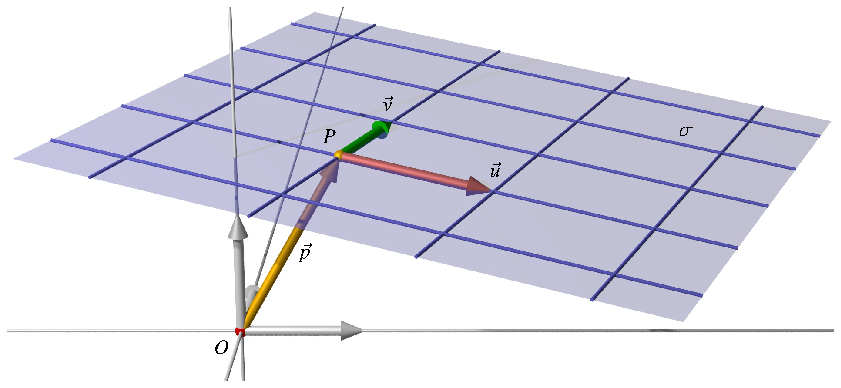
\includegraphics{3/images/ebene.pdf}
\caption{Parameterdarstellung einer Ebene $\sigma$ mit Richtungsvektoren
$\vec{u}$ und $\vec{v}$ und Stützvektor $\vec{p}$.
\label{skript:affin:ebene}}
\end{figure}
Eine Ebene erstreckt sich ausgehend von einem festen Punkt $P$ in
zwei linear unabhängige Richtungen.
Die Parameterdarstellung einer Ebene verwendet daher ausser dem
Stützvektor $\vec{p}$ zwei Richtungsvektoren $\vec{u}$ und $\vec{v}$
und braucht zwei unabhängige Parameter $t$ und $s$:
\begin{equation}
\vec{p} + t\vec{u} + s\vec{v}
\label{skript:affin:ebene:parameterdarstellung}
\end{equation}
(Abbildung~\ref{skript:affin:ebene}).

\subsubsection{Ebene durch drei Punkte}
So wie in der Ebene eine Gerade durch zwei Punkte gegeben ist, ist eine
Ebene im Raum durch drei Punkte gegeben.

\begin{aufgabe}
Gegeben sind drei Punkte $A$, $B$ und $C$, finde die Parameterdarstellung einer
Ebene durch die drei Punkte (Abbildung~\ref{skript:affin:ebene3punkte}).
\end{aufgabe}

\begin{figure}
\centering
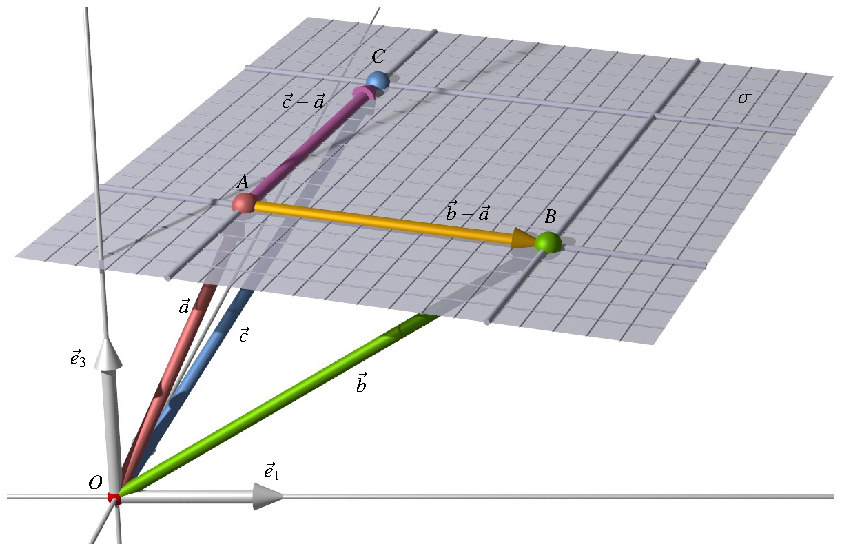
\includegraphics{3/images/ebene3punkte.pdf}
\caption{Ebene $\sigma $ durch die drei Punkte $A$, $B$ und $C$.
Als Stützvektor kann der Ortsvektor $\vec{a}$ von $A$ verwendet werden.
Die Differenzen $\vec{b}-\vec{a}$ und $\vec{c}-\vec{a}$ dienen als
Richtungsvektoren.
\label{skript:affin:ebene3punkte}}
\end{figure}
Als Stützvektor kann man jeden der drei Ortsvektoren nehmen, zum Beispiel
$\vec{a}$.
Als Richtungsvektoren kann man die Vektoren wählen, die $A$ mit $B$ bzw.~$C$
verbinden.
Daher ist eine mögliche Parameterdarstellung
\[
\vec{a} + t (\vec{b}-\vec{a}) + s(\vec{c}-\vec{a}).
\]

\begin{beispiel}
Man finde die Parameterdarstellung der Ebene durch die Punkte
$A=(1,2,1)$,
$B=(3,4,-1)$ und
$C=(4,-1,0)$.

\smallskip

{\parindent 0pt Die} Vektoren $\vec u=\overrightarrow{AB}$ und
$\vec v=\overrightarrow{AC}$ können als Richtungsvektoren
verwendet werden und ergeben als Parameterdarstellung:
\begin{equation}
\vec r=\begin{pmatrix}1\\2\\1 \end{pmatrix}
+
t\begin{pmatrix}2\\2\\-2\end{pmatrix}
+
s\begin{pmatrix}3\\-3\\-1\end{pmatrix}.
\label{beispielebene}
\qedhere
\end{equation}
\end{beispiel}

\subsubsection{Liegt ein Punkt auf einer Ebene?}
\begin{aufgabe}
Gegeben die Parameterdarstellung
\eqref{skript:affin:ebene:parameterdarstellung}
einer Ebene, entscheide, ob ein Punkt $Q$ auf der Ebene liegt.
\end{aufgabe}
Der Punkt $Q$ liegt genau dann auf der Ebene, wenn sich Parameterwerte
$t$ und $s$ finden lassen derart, dass der resultierende Vektor
der Ortsvektor $\vec{q}$ von $Q$ ist.
Dies führt auf das Gleichungssystem
\[
\vec{q}
=
\vec{p} + t\vec{u} + s\vec{v},
\]
ein Gleichungssystem mit drei Gleichung und zwei Unbekannten.
In Tableauform kann man es mit dem Gauss-Algorithmus lösen und
erhält
\[
\begin{tabular}{|>{$}c<{$}>{$}c<{$}|>{$}c<{$}|}
\hline
\color{red}t&\color{red}s&\\
\hline
u_1&v_1&q_1-p_1\\
u_2&v_2&q_2-p_2\\
u_3&v_3&q_3-p_3\\
\hline
\end{tabular}
\quad\rightarrow\quad
\begin{tabular}{|>{$}c<{$}>{$}c<{$}|>{$}c<{$}|}
\hline
\color{red}t&\color{red}s&\\
\hline
1&0&t\\
0&1&s\\
\hdashline
0&0&\color{red}*\\
\hline
\end{tabular}
\]
Der rote Stern rechts unten zeigt an, ob der Punkt $Q$ auf der Ebene liegt.
Steht dort ein von Null verschiedener Wert, hat das Gleichungssystem keine
Lösung und der Punkt $Q$ liegt nicht auf der Ebene.
In der rechten oberen Ecke kann man die Parameterwerte $t$ und $s$
ablesen, für die der Punkt $Q$ erreicht wird.

\begin{beispiel}
Liegt der Punkt $(12,9,1)$ auf der Ebene mit der Parameterdarstellung
\[
\begin{pmatrix}15\\8\\-2\end{pmatrix}
+t
\begin{pmatrix}-3\\-1\\-1\end{pmatrix}
+s
\begin{pmatrix}0\\1\\2\end{pmatrix}
?
\]
\smallskip
Wir füllen die Daten ins Tableau ein und lösen mit dem Gauss-Algorithmus:
\[
\begin{tabular}{|>{$}c<{$}>{$}c<{$}|>{$}c<{$}|}
\hline
\color{red}t&\color{red}s&\\
\hline
-3& 0&-3\\
-1& 1& 1\\
-1& 2& 3\\
\hline
\end{tabular}
\quad\rightarrow\quad
\begin{tabular}{|>{$}c<{$}>{$}c<{$}|>{$}c<{$}|}
\hline
\color{red}t&\color{red}s&\\
\hline
   1&  0&  1\\
   0&  1&  2\\
\hdashline
   0&  0&  0\\
\hline
\end{tabular}
\]
Man kann ablesen, dass der Punkt $Q$ auf der Ebene liegt und dass
er mit den Parameterwerten $t=1$ und $s=2$ erreicht wird.
\end{beispiel}

\subsubsection{Beschreiben zwei Parameterdarstellungen die gleiche Ebene?}
Die obenstehenden Beispiele haben klar gemacht, dass die gleiche Ebene
verschiedene Parameterdarstellungen haben kann.
Wie kann man entscheiden, ob zwei Parameterdarstellungen die gleiche
Ebene beschreiben?

\begin{aufgabe}
Gegeben zwei Parameterdarstellungen von Ebenen
\begin{equation*}
\sigma_1:\quad
\vec{p}_1+t\vec{u}_1+s\vec{v}_1
\qquad\text{und}\qquad
\sigma_2:\quad
\vec{p}_2+t\vec{u}_2+s\vec{v}_2,
\end{equation*}
entscheide, ob sie die gleiche Ebene beschreiben.
\end{aufgabe}
Die beiden Parameterdarstellungen beschreiben die gleiche Ebene, wenn
sich für jede Wahl der Parameter der einen Ebene ein Punkt ergibt,
der sich auch auf der zweiten Ebene befindet.
Man kann also die Vektorgleichung
\[
\vec{p}_1+t_1\vec{u}_1+s_1\vec{v}_1
=
\vec{p}_2+t_2\vec{u}_2+s_2\vec{v}_2
\]
für jede Wahl von $t_2$ und $s_2$ immer nach $t_1$ und $s_1$ auflösen.
Wir können also die Unbekannten $t_1$ und $s_1$ auf die linke Seite, die
restlichen Variablen auf die rechte schaffen und erhalten das Gleichungssystem
\[
t_1\vec{u}_1+s_1\vec{v}_1
=
\vec{p}_2-
\vec{p}_1
+t_2\vec{u}_2+s_2\vec{v}_2.
\]
In Tableauform lautet es
\[
\begin{tabular}{| >{$}c<{$} >{$}c<{$}| >{$}c<{$} >{$}c<{$} >{$}c<{$}|}
\hline
t_1&s_1&&t_2&s_2\\
\hline
u_{11}&v_{11}&p_{21}-p_{11}&u_{21}&v_{21}\\
u_{12}&v_{12}&p_{22}-p_{12}&u_{22}&v_{22}\\
u_{13}&v_{13}&p_{23}-p_{13}&u_{23}&v_{23}\\
\hline
\end{tabular}
\quad\rightarrow\quad
\begin{tabular}{| >{$}c<{$} >{$}c<{$}| >{$}c<{$} >{$}c<{$} >{$}c<{$}|}
\hline
t_1&s_1&&t_2&s_2\\
\hline
1&0&*&*&*\\
0&1&*&*&*\\
\hdashline
0&0&\color{red}*&\color{red}*&\color{red}*\\
\hline
\end{tabular}
\]
Die beiden Parameterdarstellungen beschreiben genau dann die gleiche
Ebene, wenn die {\color{red}roten} Sterne alle verschwinden.

\begin{beispiel}
Beschreiben die Parameterdarstellungen
\[
\begin{pmatrix}1 \\2 \\ 3\end{pmatrix}
+
t_1\begin{pmatrix}2\\-3\\-4\end{pmatrix}
+
s_1\begin{pmatrix}-1\\-5\\1\end{pmatrix}
\qquad\text{und}\qquad
\begin{pmatrix}1\\-11\\1\end{pmatrix}
+
t_1\begin{pmatrix}7\\-4\\-13\end{pmatrix}
+
s_1\begin{pmatrix}2\\-20\\-15\end{pmatrix}
\]
die gleiche Ebene?
\smallskip

Füllen wir die gegebenen Daten in ein Tableau ein, erhalten wir
\[
\begin{tabular}{| >{$}c<{$} >{$}c<{$}| >{$}c<{$} >{$}c<{$} >{$}c<{$}|}
\hline
t_1&s_1&&t_2&s_2\\
\hline
    2&  -1&   0&   7&   2\\
   -3&  -5& -13&  -4& -20\\
   -4&   1&  -2& -13& -15\\
\hline
\end{tabular}
\quad\rightarrow\quad
\begin{tabular}{| >{$}c<{$} >{$}c<{$}| >{$}c<{$} >{$}c<{$} >{$}c<{$}|}
\hline
t_1&s_1&&t_2&s_2\\
\hline
   1&  0&  1&  3&  4\\
   0&  1&  2& -1&  2\\
\hdashline
   0&  0&  0&  0&  1\\
\hline
\end{tabular}
\]
Die $1$ unten rechts zeigt, dass die Parameterdarstellungen nicht 
die gleiche Ebene darstellen.
\end{beispiel}
Eine weitere Möglichkeit, diese Frage zu entscheiden ist, die Schnittmenge
der beiden Ebenen zu bestimmen.
Wenn die Parameterdarstellungen die gleichen Ebene beschreiben, dann
ist die Schnittmenge wieder eine Ebene.
Wie man die Schnittmenge bestimmt, diskutieren wir im nächsten Abschnitt.

\subsection{Schnittmengen}
Die Schnittmengen von Geraden und Ebenen oder zwei Ebenen sind 
vielfältiger, können sich doch zwei Ebenen in einer Geraden
schneiden.
In diesem Abschnitt lösen wir verschiedene Schnittprobleme.

\subsubsection{Durchstosspunkt}
\begin{figure}
\centering
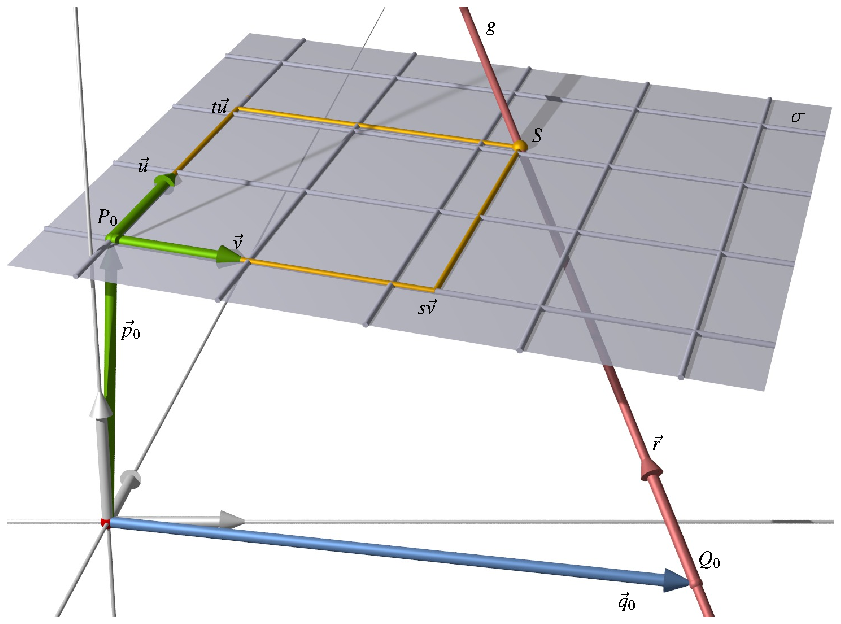
\includegraphics{3/images/durchstosspunkt.pdf}
\caption{Durchstosspunkt $S$ der Geraden $g$ durch die Ebene $\sigma$,
beide gegeben in Parameterdarstellung.
\label{skript:affin:durchstosspunkt}}
\end{figure}
Wir lösen folgende Aufgabe (siehe auch
Abbildung~\ref{skript:affin:durchstosspunkt}).

\begin{aufgabe}
Gegeben ist eine Gerade $g$ mit Parameterdarstellen
$\vec{q}_0+t\vec{r}$
und eine Ebene $\sigma$ mit Parameterdarstellung
$\vec{p}_0+t\vec{u}+s\vec{v}$.
Finde den Durchstosspunkt $S$ der Geraden $g$ durch die Ebenen $\sigma$
\end{aufgabe}

Zur Lösung der Aufgabe müssen offenbar die Streckungsfaktoren vor den
Richtungsvektoren so gefunden werden, dass sich auf der Geraden und
auf der Ebene der gleiche Punkt ergibt.
Wir müssen daher in der Geradengleichung einen unabhängigen Parameter
verwenden, zum Beispiel $w$.
Die Bedingung für den Punkt $S$ könnten wir dann als
\[
\vec{q} + w\vec{r} = \vec{p} + t\vec{u} + s\vec{v}
\]
schrieben.
Diese Vektorgleichung steht für drei Gleichungen mit den drei Unbekannten
$w$, $t$ und $s$.
Im Allgemeinen wird sie genau eine Lösung haben,
aus der durch Einsetzen in die Parameterdarstellungen die Koordinaten
des Punktes $S$ berechnet werden können.

Wie bei der Berechnung des Schnittpunktes von zwei Geraden kann man aber
auch hier schneller zum Ziel gelangen.
Wir möchten nicht nur die drei Parameter bestimmen, sondern auch gleich
die Koordinaten $x$, $y$ und $z$ des Durchstosspunktes $S$.
Wir haben die folgenden Vektorgleichungen dafür:
\[
\begin{pmatrix}x\\y\\z\end{pmatrix}
=\vec{q} + w\vec{r}
\qquad\text{und}\qquad
\begin{pmatrix}x\\y\\z\end{pmatrix}
=\vec{p} + t\vec{u} + s\vec{v}.
\]
Dies sind sechs Gleichungen für die sechs Unbekannten $x$, $y$, $z$, $t$,
$s$ und $w$.
In einem Tableau lassen sich diese Gleichungen schreiben als
\begin{equation}
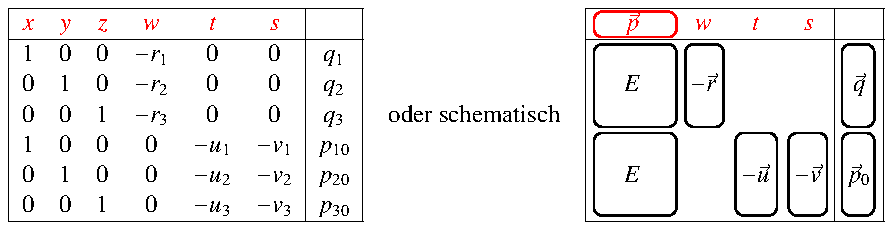
\includegraphics{3/images/durchstosspunkttableau.pdf}
\label{skript:affin:durchstosspunkttableau}
\end{equation}
Die Lösung dieses Gleichungssytems mit dem Gauss-Algorithmus
gibt in einem Durchgang alle gesuchten Grössen.

\begin{beispiel}
Finde den Durchstosspunkt der Geraden mit Parameterdarstellung
\[
\begin{pmatrix} 5\\8\\3 \end{pmatrix}
+
w\begin{pmatrix} 1\\0\\1 \end{pmatrix}
\]
durch die Ebene mit Parameterdarstellung
\[
\begin{pmatrix}1\\2\\1 \end{pmatrix}
+
t\begin{pmatrix}2\\2\\-2\end{pmatrix}
+
s\begin{pmatrix}3\\-3\\-1\end{pmatrix}.
\]
Einsetzen ins Tableau~\ref{skript:affin:durchstosspunkttableau}
und Lösen mit dem Gaussalgorithmus liefert
\[
\begin{tabular}{|>{$}c<{$}>{$}c<{$}>{$}c<{$}>{$}c<{$}>{$}c<{$}>{$}c<{$}|>{$}c<{$}|}
\hline
\color{red}x&\color{red}y&\color{red}z&\color{red}w&\color{red}t&\color{red}s&\\
\hline
1&0&0&-1& 0& 0&5\\
0&1&0& 0& 0& 0&8\\
0&0&1&-1& 0& 0&3\\
1&0&0& 0&-2&-3&1\\
0&1&0& 0&-2& 3&2\\
0&0&1& 0& 2& 1&1\\
\hline
\end{tabular}
\quad\rightarrow\quad
\begin{tabular}{|>{$}c<{$}>{$}c<{$}>{$}c<{$}>{$}c<{$}>{$}c<{$}>{$}c<{$}|>{$}c<{$}|}
\hline
\color{red}x&\color{red}y&\color{red}z&\color{red}w&\color{red}t&\color{red}s&\\
\hline
1&0&0& 0& 0& 0& 1\\
0&1&0& 0& 0& 0& 8\\
0&0&1& 0& 0& 0&-1\\
0&0&0& 1& 0& 0&-4\\
0&0&0& 0& 1& 0& \frac32\\
0&0&0& 0& 0& 1&-1\\
\hline
\end{tabular}
\]
Daraus kann man ablesen, dass der Durchstosspunkt $S$ die Koordinaten
$(1,8,-1)$ hat, die für die Parameterwerte $w=-4$, $t=\frac32$ und $s=-1$
erreicht werden.
\end{beispiel}

\subsubsection{Schnittgerade}
\begin{figure}
\centering
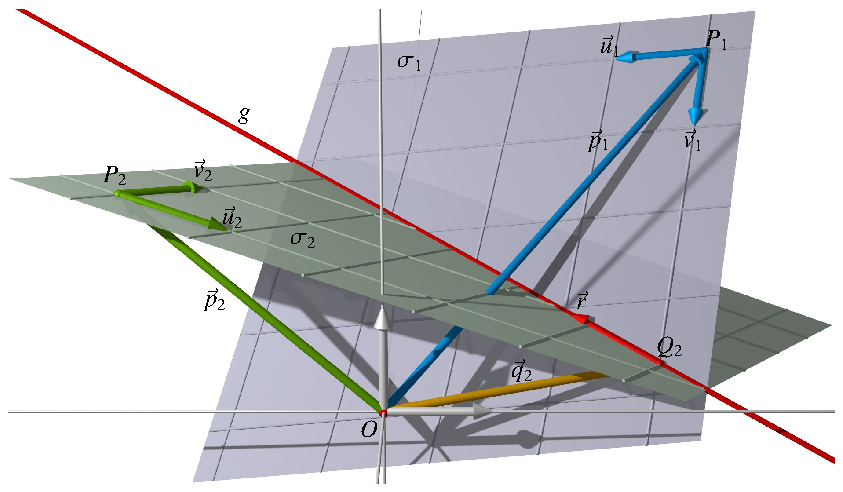
\includegraphics{3/images/schnittgerade.pdf}
\caption{Schnittgerade $g$ zweier Ebenen $\sigma_1$ und $\sigma_2$, beide
gegeben in Parameterdarstellung.
\label{skript:affin:schnittgerade}}
\end{figure}
Zwei Ebenen schneiden sich im dreidimensionalen Raum typischerweise in 
einer Geraden.
Diese zu finden, ist der Inhalt der folgenden Aufgabe

\begin{aufgabe}
\label{skript:affin:aufgabe:schnittgerade}
Gegeben zwei Ebenen $\sigma_1$ und $\sigma_2$ mit Parameterdarstellungen
\begin{equation}
\sigma_1:\quad
\vec{p}_1+t\vec{u}_1+s\vec{v}_1
\qquad\text{und}\qquad
\sigma_2:\quad
\vec{p}_2+t\vec{u}_2+s\vec{v}_2,
\label{skript:affin:aufgabe:schnittgerade:gleichungen}
\end{equation}
finde die Schnittgerade $g=\sigma_1\cap\sigma_2$ mit der Parameterdarstellung
\[
\vec{p}
=
\vec{q}
+
t\vec{r.}
\]
(siehe auch Abbildung~\ref{skript:affin:schnittgerade})
\end{aufgabe}

Wir stellen ein Gleichungssystem auf für die Unbekannten $t_1$,
$s_1$, $t_2$ und $s_2$ sowie die unbekannten Komponenten des Vektors
\[
\vec{p}
=\begin{pmatrix} x\\y\\z\end{pmatrix}.
\]
Die Ebenengleichungen in Tableauform werden zu
\begin{equation}
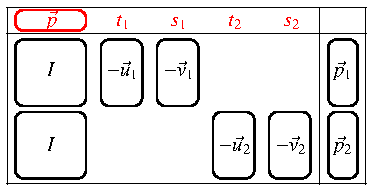
\includegraphics{3/images/schnittgeradetableau.pdf}
\label{skript:affin:schnittgeradetableau}
\end{equation}
Dies sind sechs Gleichungen für sieben Unbekannte.
Im allgemeinen Fall wird das Schlusstableau daher die Form
\begin{equation}
\begin{tabular}{|
>{$}c<{$}
>{$}c<{$}
>{$}c<{$}
>{$}c<{$}
>{$}c<{$}
>{$}c<{$}
>{$}c<{$}|
>{$}c<{$}|}
\hline
\color{red}x&
\color{red}y&
\color{red}z&
\color{red}t_1&
\color{red}s_1&
\color{red}t_2&
\color{red}s_2&\\
\hline
1&0&0&0&0&0&-r_1&q_1\\
0&1&0&0&0&0&-r_2&q_2\\
0&0&1&0&0&0&-r_3&q_3\\
0&0&0&1&0&0&-r_4&q_4\\
0&0&0&0&1&0&-r_5&q_5\\
0&0&0&0&0&1&-r_6&q_6\\
\hline
\end{tabular}
\label{skript:affin:schnittgerade:schlusstableau}
\end{equation}
haben.
Daraus kann man zunächst die Parameterdarstellung der Schnittgerade
ablesen:
\[
\begin{pmatrix}x\\y\\z\end{pmatrix}
=
\begin{pmatrix}q_1\\q_2\\q_3\end{pmatrix}
+
s_2\begin{pmatrix}r_1\\r_2\\r_3\end{pmatrix}.
\]
Man kann in den letzten drei Gleichungen auch ablesen, wie die Parameter
$t_1$, $s_1$ und $t_2$ von $s_2$ abhängen für Punkte, die auf der
Schnittgeraden liegen, nämlich
\begin{align*}
t_1&=q_4+s_2r_4,&
s_1&=q_5+s_2r_5&
&\text{und}&
t_2&=q_6+s_2r_6.
\end{align*}
Dieses Verfahren liefert also alle Informationen, die man über dieses
Problem in Erfahrung bringen kann.

\begin{beispiel}
Man finde die Schnittgerade der beiden Ebenen mit Parameterdarstellung
\[
\sigma_1:
\vec p_1+t_1\vec u_1+s_1\vec v_1
=\begin{pmatrix}5\\8\\6\end{pmatrix}
+t_1\begin{pmatrix}4\\6\\7\end{pmatrix}
+s_1\begin{pmatrix}2\\5\\6\end{pmatrix}
,
\qquad
\sigma_2:
\vec p_2+t_2\vec u_2+s_2\vec v_2
=\begin{pmatrix}5\\4\\4\end{pmatrix}
+t_2\begin{pmatrix}6\\6\\7\end{pmatrix}
+s_2\begin{pmatrix}5\\4\\4\end{pmatrix}.
\]
Das zugehörige Tableau ist
\[
\begin{tabular}{|
>{$}c<{$}
>{$}c<{$}
>{$}c<{$}
>{$}c<{$}
>{$}c<{$}
>{$}c<{$}
>{$}c<{$}|
>{$}c<{$}|}
\hline
\color{red}x&
\color{red}y&
\color{red}z&
\color{red}t_1&
\color{red}s_1&
\color{red}t_2&
\color{red}s_2&\\
\hline
1&0&0&-4&-2& 0& 0&5\\
0&1&0&-6&-5& 0& 0&8\\
0&0&1&-7&-6& 0& 0&6\\
1&0&0& 0& 0&-6&-5&5\\
0&1&0& 0& 0&-6&-4&4\\
0&0&1& 0& 0&-7&-4&4\\
\hline
\end{tabular}
\quad\rightarrow\quad
\begin{tabular}{|
>{$}c<{$}
>{$}c<{$}
>{$}c<{$}
>{$}c<{$}
>{$}c<{$}
>{$}c<{$}
>{$}c<{$}|
>{$}c<{$}|}
\hline
\color{red}x&
\color{red}y&
\color{red}z&
\color{red}t_1&
\color{red}s_1&
\color{red}t_2&
\color{red}s_2&\\
\hline
1&0&0&0&0&0&-14        &-67\\
0&1&0&0&0&0&-13        &-68\\
0&0&1&0&0&0&-\frac{29}2&-80\\
0&0&0&1&0&0&-\frac{11}2&-26\\
0&0&0&0&1&0&4          & 16\\
0&0&0&0&0&1&-\frac{3}2 &-12\\
\hline
\end{tabular}
\]
Daraus kann man die Parameterdarstellung
\[
\begin{pmatrix} x\\y\\z\end{pmatrix}
=
\begin{pmatrix}-67\\-68\\-80\end{pmatrix}
+s_2\begin{pmatrix}14\\13\\\frac{29}2\end{pmatrix}
\]
der Schnittgeraden ablesen.
\end{beispiel}

Falls bei der Lösung des Gleichungssystems zwei frei wählbare Variablen stehen
bleiben können wir schliessen, dass die Schnittmenge eine Ebene ist.
Dies ist nur möglich, wenn die beiden Parameterdarstellungen die
gleiche Ebene beschreiben.

\subsubsection{Schnittpunkt zweier Ebenen im vierdimensionalen Raum}
Die Vektorgeometrie eröffnet uns die Möglichkeit, Probleme zu lösen,
die wir graphisch nicht visualisieren können und uns nicht vorstellen
können.
Wir können uns zum Beispiel fragen, wie die Schnittmenge von zwei Ebenen
in einem vierdimensionalen Raum aussieht.
Die Parameterdarstellung
\eqref{skript:affin:aufgabe:schnittgerade:gleichungen}
der Ebenen
in Aufgabe~\ref{skript:affin:aufgabe:schnittgerade}
ändert nicht.
Die Vektoren sind neu einfach vierdimensionale Vektoren.
Auch das Tableau~\eqref{skript:affin:schnittgeradetableau} bleibt gleich,
stellt jetzt aber 8 Gleichungen für 8 Unbekannte dar.
Das Schlusstableau hat also im Allgemeinen die Form
\[
\begin{tabular}{|
>{$}c<{$}
>{$}c<{$}
>{$}c<{$}
>{$}c<{$}
>{$}c<{$}
>{$}c<{$}
>{$}c<{$}
>{$}c<{$}|
>{$}c<{$}|}
\hline
\color{red}x&
\color{red}y&
\color{red}z&
\color{red}t&
\color{red}t_1&
\color{red}s_1&
\color{red}t_2&
\color{red}s_2&
\\
\hline
1&0&0&0&0&0&0&0&p_1\\
0&1&0&0&0&0&0&0&p_2\\
0&0&1&0&0&0&0&0&p_3\\
0&0&0&1&0&0&0&0&p_4\\
0&0&0&0&1&0&0&0&p_5\\
0&0&0&0&0&1&0&0&p_6\\
0&0&0&0&0&0&1&0&p_7\\
0&0&0&0&0&0&0&1&p_8\\
\hline
\end{tabular}\,,
\]
woraus man den Schnittpunkt  $(p_1,p_2,p_3,p_4)$ ablesen kann.
Zwei Ebenen im vierdimensionalen Raum schneiden sich also im Allgemeinen
in einem Punkt, ganz ähnlich wie sich zwei Geraden in einer Ebene in
einem Punkt schneiden.

\subsection{Ebenen und lineare Abbildungen}
\subsubsection{Ebene als Bild einer linearen Abbildung}
\begin{figure}
\centering
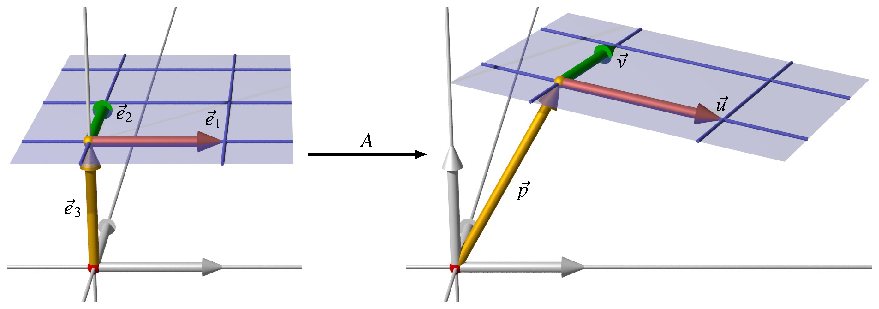
\includegraphics{3/images/abb.pdf}
\caption{Ebene als Abbildung einer Standardebene mit $\vec{e}_1$ und
$\vec{e}_2$ als Richtungsvektoren und $\vec{e}_3$ als Stützvektor.
\label{skript:affin:ebeneabb}}
\end{figure}
Wie eine Gerade kann auch eine Ebene als Bild einer Standardebene
unter einer linearen Abbildung betrachtet werden.
Die Abbildung muss $\vec{e}_1$ auf den ersten Richtungsvektor,
$\vec{e}_2$ auf den zweiten Richtungsvektor und $\vec{e}_3$ auf den
Stützvektor abbilden.
Die Abbildungsmatrix muss also in der ersten Spalte den Richtungsvektor
$\vec{u}$ enthalten, in der zweiten den Richtungsvektor $\vec{v}$ und in
der dritten Spalten den Stütztvektor $\vec{p}$, wie in
\[
A=\begin{pmatrix}
u_1&v_1&p_1\\
u_2&v_2&p_2\\
u_3&v_3&p_3\\
\end{pmatrix}.
\]
Die Parameterdarstellung kann dann wieder in Matrixform geschrieben werden
als
\[
t\vec{u}+s\vec{v}+\vec{p}
=
A
\begin{pmatrix}t\\s\\1\end{pmatrix}
=
\begin{pmatrix}
u_1&v_1&p_1\\
u_2&v_2&p_2\\
u_3&v_3&p_3\\
\end{pmatrix}
\begin{pmatrix}t\\s\\1\end{pmatrix}.
\]

\subsubsection{Ebene im Raum als Nullmenge}
Wir bestimmen die Lösungsmenge einer einzelnen linearen Gleichung
\begin{equation}
ax+by+cz=d
\label{skript:affin:ebene:nullmenge}
\end{equation}
der drei Koordinaten $x$, $y$ und $z$ des dreidimensionalen Raumes.
Das Gauss-Tableau hat die Form
\[
\begin{tabular}{|>{$}c<{$}>{$}c<{$}>{$}c<{$}|>{$}c<{$}|}
\hline
x&y&z&\\
\hline
a&b&c&d\\
\hline
\end{tabular}
\quad\rightarrow\quad
\begin{tabular}{|>{$}c<{$}>{$}c<{$}>{$}c<{$}|>{$}c<{$}|}
\hline
x&y&z&\\
\hline
1&\frac{b}{a}&\frac{c}{a}&\frac{d}{a}\\
\hline
\end{tabular}
\]
Man hat also zwei frei wählbare Variablen, nämlich $y$ und $z$, und
man kann die Lösungsmenge schreiben als
\[
\mathbb L
=
\left\{
\left.
\begin{pmatrix}\frac{d}{a}\\0\\0 \end{pmatrix}
+
y\begin{pmatrix}-\frac{b}{a}\\1\\0\end{pmatrix}
+
z\begin{pmatrix}-\frac{c}{a}\\0\\1\end{pmatrix}
\;
\right|
\;
x,y\in\mathbb R
\right\}
\]
In der Megenklammer steht die Parameterdarstellung einer Ebene.


Umgekehrt kann man auch zu einer beliebigen Ebene mit Parameterdarstellung
\[
\vec{p}+t\vec{u}+s\vec{v}
\]
eine lineare Gleichung finden, die die Ebene als Lösungemenge hat.
Dazu setzt man die Gleichung in der
Form~\eqref{skript:affin:ebene:nullmenge} an und setzt die drei
Punkte $\vec{p}$, $\vec{p}+\vec{u}$ und $\vec{p}+\vec{v}$ ein:
\[
\begin{linsys}{3}
p_1a&+&p_2b&+&p_3c&=&d\\
(p_1+u_1)a&+&(p_2+u_2)b&+&(p_3+u_3)c&=&d\\
(p_1+v_1)a&+&(p_2+v_2)b&+&(p_3+v_3)c&=&d\\
\end{linsys}
\]
Wir bringen die Unbekannte $d$ ebenfalls auf die linke Seite und schreiben
das in Tableauform als
\begin{align}
\begin{tabular}{|>{$}c<{$}>{$}c<{$}>{$}c<{$}>{$}c<{$}|>{$}c<{$}|}
\hline
a&b&c&d&\\
\hline
p_1&p_2&p_3&-1&0\\
p_1+u_1&p_2+u_2&p_3+u_3&-1&0\\
p_1+v_1&p_2+v_2&p_3+v_3&-1&0\\
\hline
\end{tabular}
&\rightarrow
\begin{tabular}{|>{$}c<{$}>{$}c<{$}>{$}c<{$}>{$}c<{$}|>{$}c<{$}|}
\hline
a&b&c&d&\\
\hline
p_1&p_2&p_3&-1&0\\
u_1&u_2&u_3& 0&0\\
v_1&v_2&v_3& 0&0\\
\hline
\end{tabular}
\label{skript:affin:ebene:abcd}
\\
&\rightarrow
\begin{tabular}{|>{$}c<{$}>{$}c<{$}>{$}c<{$}>{$}c<{$}|>{$}c<{$}|}
\hline
a&b&c&d&\\
\hline
1&0&0&a_1&0\\
0&1&0&b_1&0\\
0&0&1&c_1&0\\
\hline
\end{tabular}
\notag
\end{align}
Die Variable $d$ ist frei wählbar, die anderen erhält man mittels
$a=-a_1d$, $b=-b_1d$ und $c=-c_1d$.

\begin{beispiel}
Man finde eine lineare Gleichung, deren Lösungsmenge die Ebene mit der
Parameterdarstellung
\[
\begin{pmatrix}-3\\1\\-2\end{pmatrix}
+t
\begin{pmatrix}-4\\-5\\-3\end{pmatrix}
+s
\begin{pmatrix} 3\\-2\\ 2\end{pmatrix}
\]
ist.

\smallskip

{\parindent=0pt Wir} füllen diese Information in des Tableau~\eqref{skript:affin:ebene:abcd}
\[
\begin{tabular}{|
>{$}c<{$}
>{$}c<{$}
>{$}c<{$}
>{$}c<{$}|
>{$}c<{$}|}
\hline
a&b&c&d&\\
\hline
  -3&  1& -2& -1&  0\\
  -4& -5& -3&  0&  0\\
   3& -2&  2&  0&  0\\
\hline
\end{tabular}
\rightarrow
\begin{tabular}{|
>{$}c<{$}
>{$}c<{$}
>{$}c<{$}
>{$}c<{$}|
>{$}c<{$}|}
\hline
a&b&c&d&\\
\hline
    1&   0&   0&  16&  0\\
    0&   1&   0&   1&   0\\
    0&   0&   1& -23&   0\\
\hline
\end{tabular}
\]
und leiten daraus mit der willkürlichen Wahl $d=1$ 
\[
a=-16d=-16,
\quad
b=-d=-1,
\quad
c=23d=23
\]
und damit die Gleichung
\[
-16x-y+23z=1
\]
ab.
Sie hat als Lösungsmenge die gegebene Ebene.
\end{beispiel}

